\documentclass[11pt, letterpaper]{article}
\usepackage[margin=0.8in]{geometry}
\usepackage[utf8]{inputenc}
\usepackage{graphicx}

\title{AI Isolation Game-playing Agent Report}
\author{Jiyao Li}
\date{February 20, 2017}
 
\begin{document}
	\maketitle 
	
In this project, after making my code working with minimax search, alpha-beta pruning, depth-limited and iterative deepening search, I explored several Heuristic scoring functions. 

The three proved evaluation Heuristic functions are NullEval, OpenMoveEval and ImprovedEval. NullEval returns 0 when not wining or losing. OpenMoveEval use ``number of my moves'' as heuristic evaluation. ImprovedEval use ``number of my moves - number of opponent moves'' as evaluation function.

I created 3 Heuristic scoring functions, all of which achieved better Elo score compared with the ID\_Improved agent when playing against the seven reference agents (Random, Minimax with NullEval, Minimax with OpenMoveEval, Minimax with ImprovedEval, Alpha-beta with NullEval, Alpha-beta with OpenMoveEval, Alpha-beta with ImprovedEval). The Minimax and Alpha-beta search in the reference agents are implemented as depth-limited search. 

When making my own evaluation functions, I tried to make them fast and nice, rather than complicated and slow. As we know, slow and sophisticated evaluation function may provide more accurate evaluation of which is the next best move for tree with specific levels. But it will consume time and prevent deeper tree search. My Student Heuristic evaluation functions are:

Student H1 Agent: ``number of my moves - 2 $\times$ number of opponent moves''. This evaluation function was mentioned in the lecture video. The idea is to penalize the opponent even more. 

Student H2 Agent: ``(number of my moves - number of opponent moves) $\times$ number of occupied spaces''. From testing, I agree that ``number of my moves - number of opponent moves'' is a nice and simple Heuristic function. And I think that toward the end of the game when there are not many empty spaces left, if my agent is still likely to win, the chance must be higher. For example, if in the very beginning of the game. My agent has 8 possible moves while my opponent has 7 possible moves. Toward the end of the game, if ``number of my moves - number of opponent moves'' is still 1, my agent will be more likely to win since there are not many moves left. So I use the ``time left'' to the end of the game as a weighting factor.

Student H3 Agent: ``(number of my moves - number of opponent moves) $\times$ Manhattan distance between my agent and the opponent''. Here I used another weighting factor, Manhattan distance between the two agents. The idea is that if the two agents are separated far, then it will be less likely for them to interfere with each other. So the one with more possible moves will more likely win. If they are close to each other, then they will occupy each other's future position. And whether one with more current possible next move will win is less clear.

Become of many randomness involved in the tournament, e.g. the first step is taken randomly, the Elo scores are not quite stable. So I ran the tournament two times. Each time, there are in total 20 matches between two agents. Table \ref{table1} shows the averaged Elo score of DI\_Improved agents and my Student agents VS other reference agents. All of my three Heuristic evaluation functions outperform the DI\_Improved agent. And ``Student H1'' agent got the highest score. Thus I will recommend using that one. 

Figure \ref{figure1} shows itemized wining ratio of ID\_Improved agents and my three Student agent playing against the seven reference agent. 

\begin{table}[h!]
	\centering
	\caption{Overall winning ratio.}
	\label{table1}
	\begin{tabular}{| c | c | c |c |c |}
		\hline
		User-Agent & DI\_Improved & Student H1 & Student H2 & Student H3 \\
		\hline
		Overall Win ratio & 64.64\% &69.29\% & 68.58\% & 68.57\% \\
		\hline
	\end{tabular}
\end{table}

\begin{figure}[h!]
	\centering
	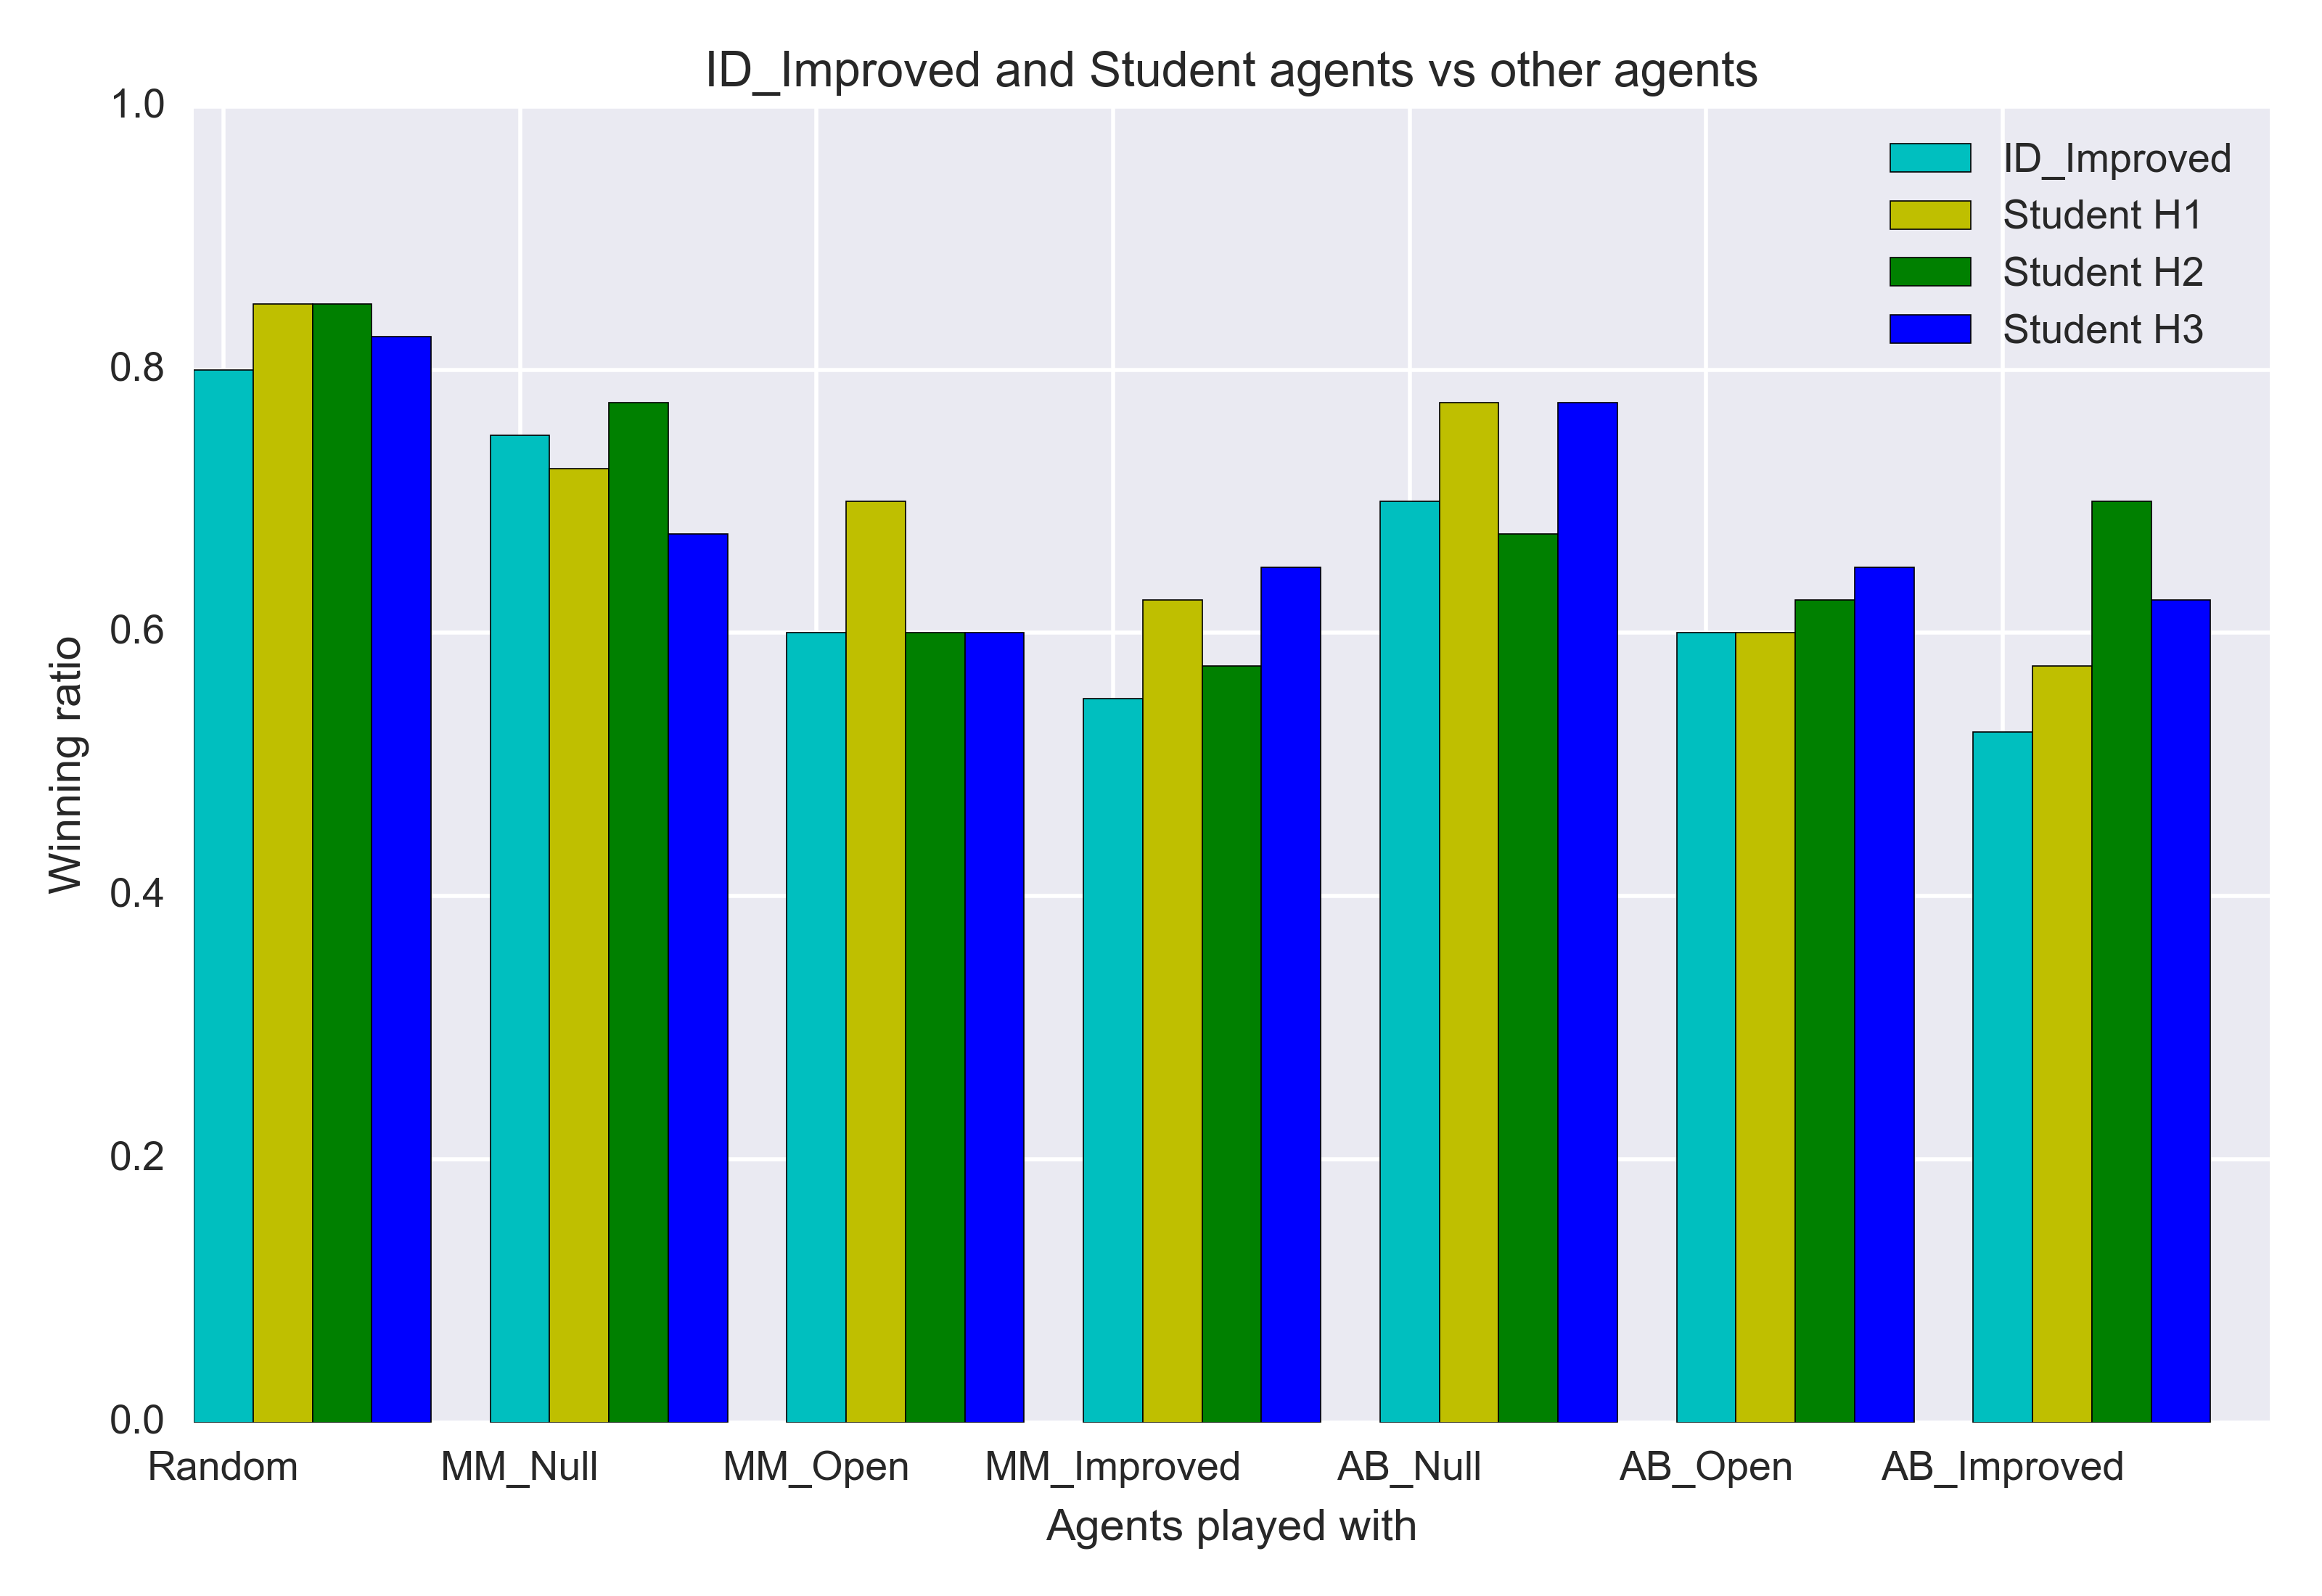
\includegraphics[width=6.5in]{bar_student3agent.png}
	\caption{Itemized winning ratio of ID\_Improved agent, three Student agents playing with Random, MN\_Null, MN\_Open, MN\_Improved, Ab\_Null, Ab\_Open, Ab\_Improved agents.}
	\label{figure1}
\end{figure}

\end{document}